% !TEX program = lualatex
\documentclass[final]{beamer}

% ====================
% Pacotes
% ====================

\usepackage[T1]{fontenc}
\usepackage{lmodern}
\usepackage[orientation=portrait,size=a0,scale=1.2]{beamerposter}
\usepackage[english]{babel}
\usepackage{amsmath, amssymb}
\usepackage{graphicx}
\usepackage{booktabs}

\usetheme{gemini}
\usecolortheme{labfluid}

% ====================
% Configurações de Layout
% ====================

\newlength{\sepwidth}
\newlength{\colwidth}
\setlength{\sepwidth}{0.04\paperwidth}
\setlength{\colwidth}{0.44\paperwidth}

\newcommand{\separatorcolumn}{\begin{column}{\sepwidth}\end{column}}

% ====================
% Informações do Cabeçalho
% ====================

\title{Physics-Informed Neural Networks for Numerical Approximations of the Boussinesq System of Partial Differential Equations}
\author{Samuel Kutz Paranhos \\[1ex] Prof. Roberto Ribeiro}

\institute{\normalsize PIBIC 2024}



\setlength{\fboxsep}{8pt} % Adiciona um "padding" à caixa branca

% Ajuste das Logos Laterais
\logoleft{%
  % The [s] option at the end allows \vfill to distribute the vertical space
  \begin{minipage}[c][16cm][s]{15cm} 
    \centering
    % Upper-left logo
    
\includegraphics[height=8cm,keepaspectratio]{imgs/brasao_UFSC.png}
    \vfill % Pushes the next image to the bottom
    
    % Lower-left logo
    
\includegraphics[height=11cm,keepaspectratio]{imgs/BrazOpt_LOGO.png}
  \end{minipage}
}

\logoright{%
  \begin{minipage}[c][16cm][s]{15cm}
    \centering
    \vspace{2.5cm}
    % Upper-right logo
    
\includegraphics[height=3cm,keepaspectratio]{imgs/CNPq.png} 
    \vspace{2.4cm} % Pushes the next image to the bottom
    
    % Lower-right logo
    
\includegraphics[height=11cm,keepaspectratio]{imgs/LabFluidLogo.png}
  \end{minipage}
}

% ====================
% Início do Documento
% ====================

\begin{document}


\begin{frame}[t]
\begin{columns}[t]
\separatorcolumn

% --------------------
% --- COLUNA 1 -------
% --------------------
\begin{column}{\colwidth}

  \begin{block}{Introduction}
    This work investigates \textcolor{UniBlue}{Physics-Informed Neural Networks (PINNs)}, a \textit{Deep Learning}-based alternative that approximates solutions of Partial Differential Equations (PDEs) in a continuous manner by incorporating the PDE directly into the neural network loss function during training \cite{raissi2017}, as a regularization term.

    The objective is therefore to assess the performance of this approach in solving the simplified Boussinesq system, a nonlinear model for simulating shallow water waves.
  \end{block}

  \begin{block}{Physics-Informed Neural Networks (PINNs)}
    PINNs adapt the neural network architecture (in this case, \textit{Multilayer Perceptrons}, MLPs) to find approximate solutions of PDE instances. The method aims to solve a generic system, written in terms of a differential operator $\mathcal{D}$:
    \begin{equation*}
        \left\{
        \begin{aligned}
            & \mathcal{D}[u](x,t) = 0, \quad \forall (x,t) \in \Omega \times (0, T] \\
            & u(x,0) = u_0(x), \quad x \in \Omega
        \end{aligned}
        \right.
    \end{equation*}
    The network is trained to minimize the Mean Squared Error (MSE), combining the physics and initial-condition errors:
    \begin{equation*}
    \resizebox{0.9\columnwidth}{!}{ $
    \text{MSE}(\theta) = \underbrace{\frac{1}{N_{\mathcal{D}}} \sum_{i=1}^{N_{\mathcal{D}}} \left( \mathcal{D}[u_\theta](x_i, t_i) \right)^2}_{\text{PDE residual}} +
                       \underbrace{\frac{1}{N_{0}} \sum_{j=1}^{N_{0}} \left( u_\theta(x_j, 0) - u_0(x_j) \right)^2}_{\text{Initial condition}}
    $ }
    \end{equation*}
    where $\{x_i, t_i\}_{i=1}^{N_{\mathcal{D}}}$ are the collocation points inside the domain and $\{x_j\}_{j=1}^{N_0}$ are the collocation points sampled on the initial condition. These points are usually sampled from uniform distributions over the PDE domain.
  \end{block}
  \begin{block}{The Boussinesq System}
    This system describes wave propagation in shallow waters, modeling the evolution of the free-surface elevation, $\eta(x,t)$, and the depth-averaged horizontal velocity, $u(x,t)$: 
    \begin{equation*}
    \left\{
    \begin{aligned}
        & \eta_t + u_x + \alpha(\eta u)_x = 0, \qquad \text{for } (x,t) \in [-30, 30] \times [0, 15] \\
        & u_t + \eta_x + \alpha u u_x - \tfrac{\beta}{3} u_{xxt} = 0, \\
        % & \eta(x, 0) = \text{sech}^2(x), \\
        % & u(x, 0) = 0.
    \end{aligned}
    \right.
    \end{equation*}
    where $\alpha$ and $\beta$ are parameters that control the effects of nonlinearity and dispersion. In our study, we solve this problem subject to the initial condition
    \begin{equation*}
    \begin{aligned}
        & \eta(x, 0) = \text{sech}^2(x), \\
        & u(x, 0) = 0.
    \end{aligned}
    \end{equation*}

    These initial conditions are chosen because, in the case $\alpha = \beta = 0$, the solution to this problem can be determined exactly by D'Alembert's formula, making it a good test for PINNs. Otherwise, effectiveness is tested by comparison with the solution obtained from the pseudospectral method.
  \end{block}
  
  \begin{block}{Spectral Bias and Adaptive Sampling}
    A known difficulty in PINNs is Spectral Bias \cite{rahaman2019spectral}, a tendency of MLP neural networks to learn the low-frequency components of the solution first. In order to mitigate this effect, we implement the adaptive sampling strategy \textit{Residual-based Adaptive Refinement} (RAR) \cite{wu2023comprehensive}, which consists of abandoning the uniform point distribution and sampling new points based on a probability density $p(x)$ that prioritizes regions with higher error (PDE residual, $|\mathcal{D}[u_\theta](x,t)|$). 
    
    In RAR, for parameters $ k, c \geq 0 $, the probability density function has the form (subject to normalization):
    \begin{equation*}
        p(x) \propto \frac{|\mathcal{D}[u_\theta](x,t)|^k}{\mathbb{E}[|\mathcal{D}[u_\theta](x,t)|^k]} + c.
    \end{equation*}
   This leads the network to prioritize allocating points where the residual is larger (where it is making more errors), as shown in Figure \ref{fig:sampling_dist}.
    \begin{figure}
        \centering
        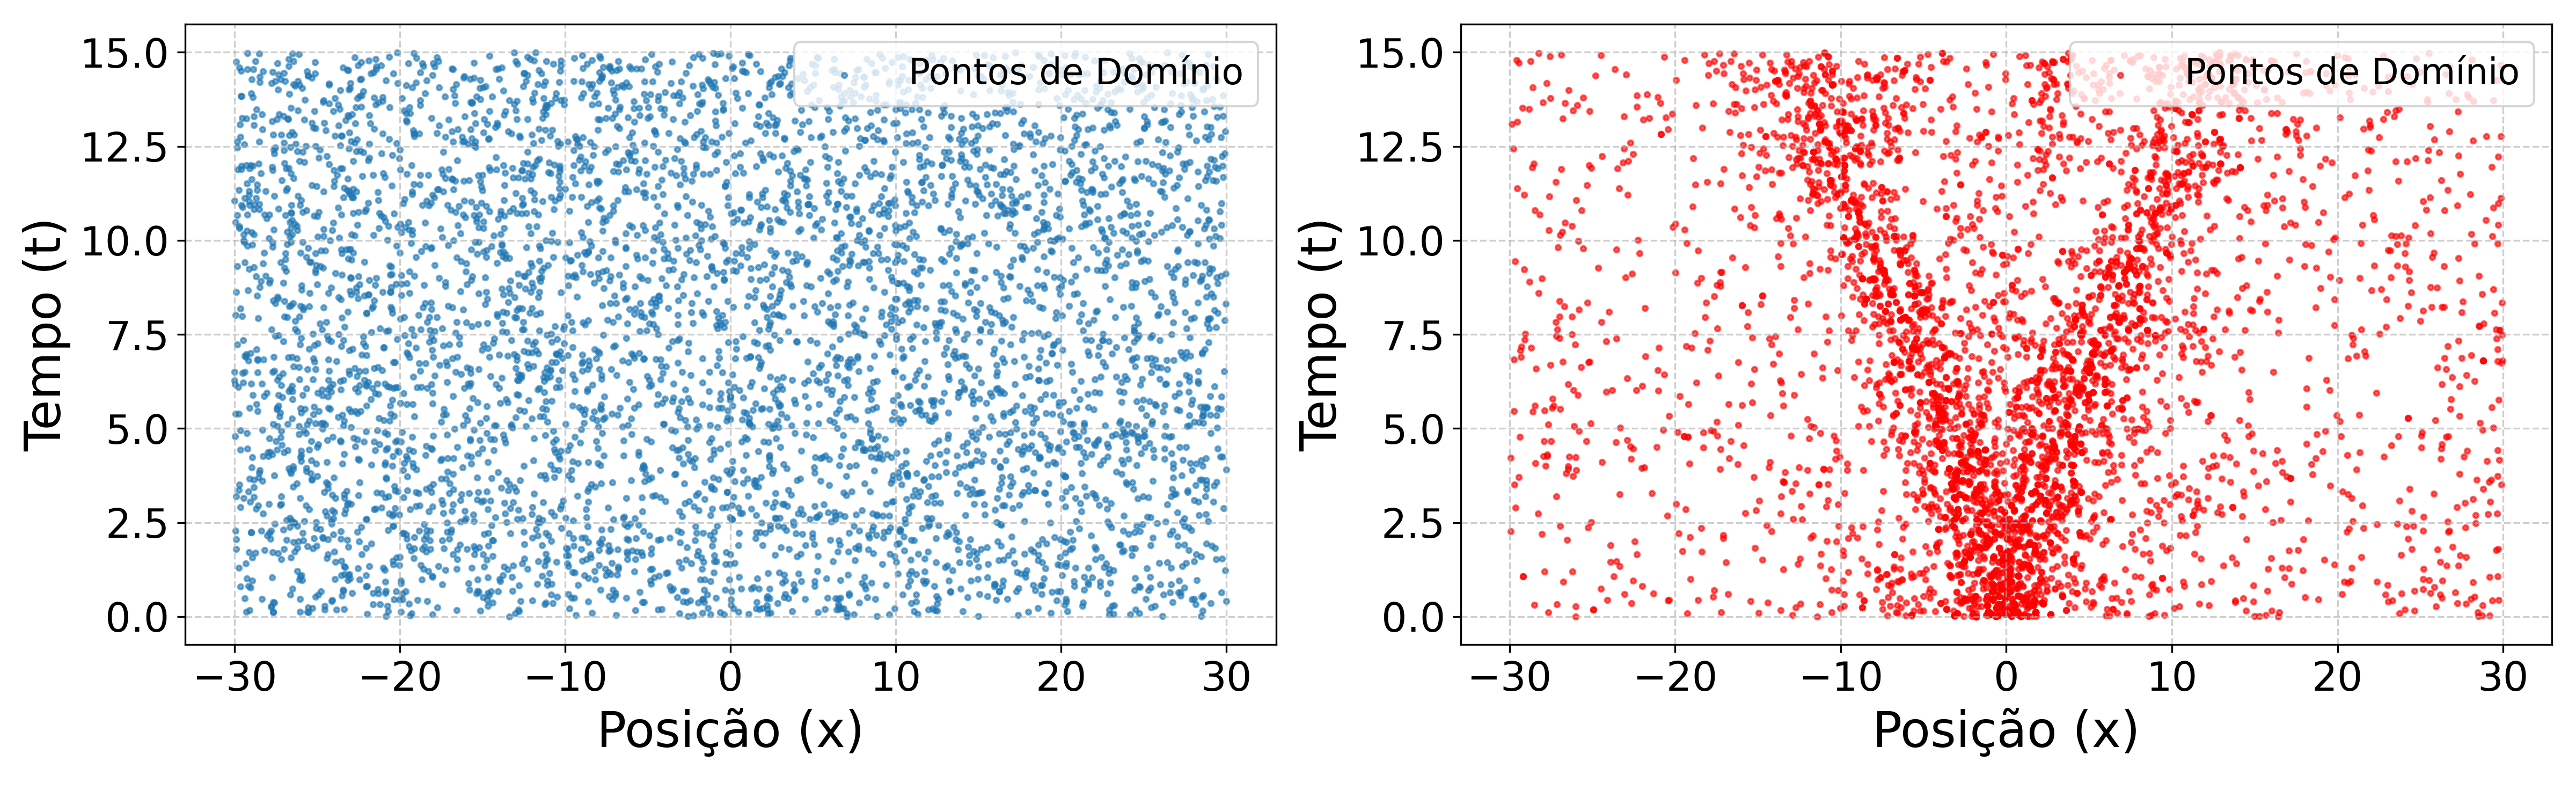
\includegraphics[width=\columnwidth]{imgs/rar_point_distribution_comparison.png}
        \caption{Point distribution: uniform (left) vs. adaptive with RAR (right).}        
        \label{fig:sampling_dist}
   \end{figure}

  \end{block}
\end{column}

\separatorcolumn

% --------------------
% --- COLUNA 2 -------
% --------------------
\begin{column}{\colwidth}
    \begin{block}{Results and Discussion}
        The PINN was tested in scenarios of increasing complexity, although still relatively simple, with $\alpha=\beta=10^{-4}$ and $\alpha=\beta=10^{-1}$ - regimes that are still not very complex, but sufficient to observe some important points:
        \begin{figure}
            \centering
            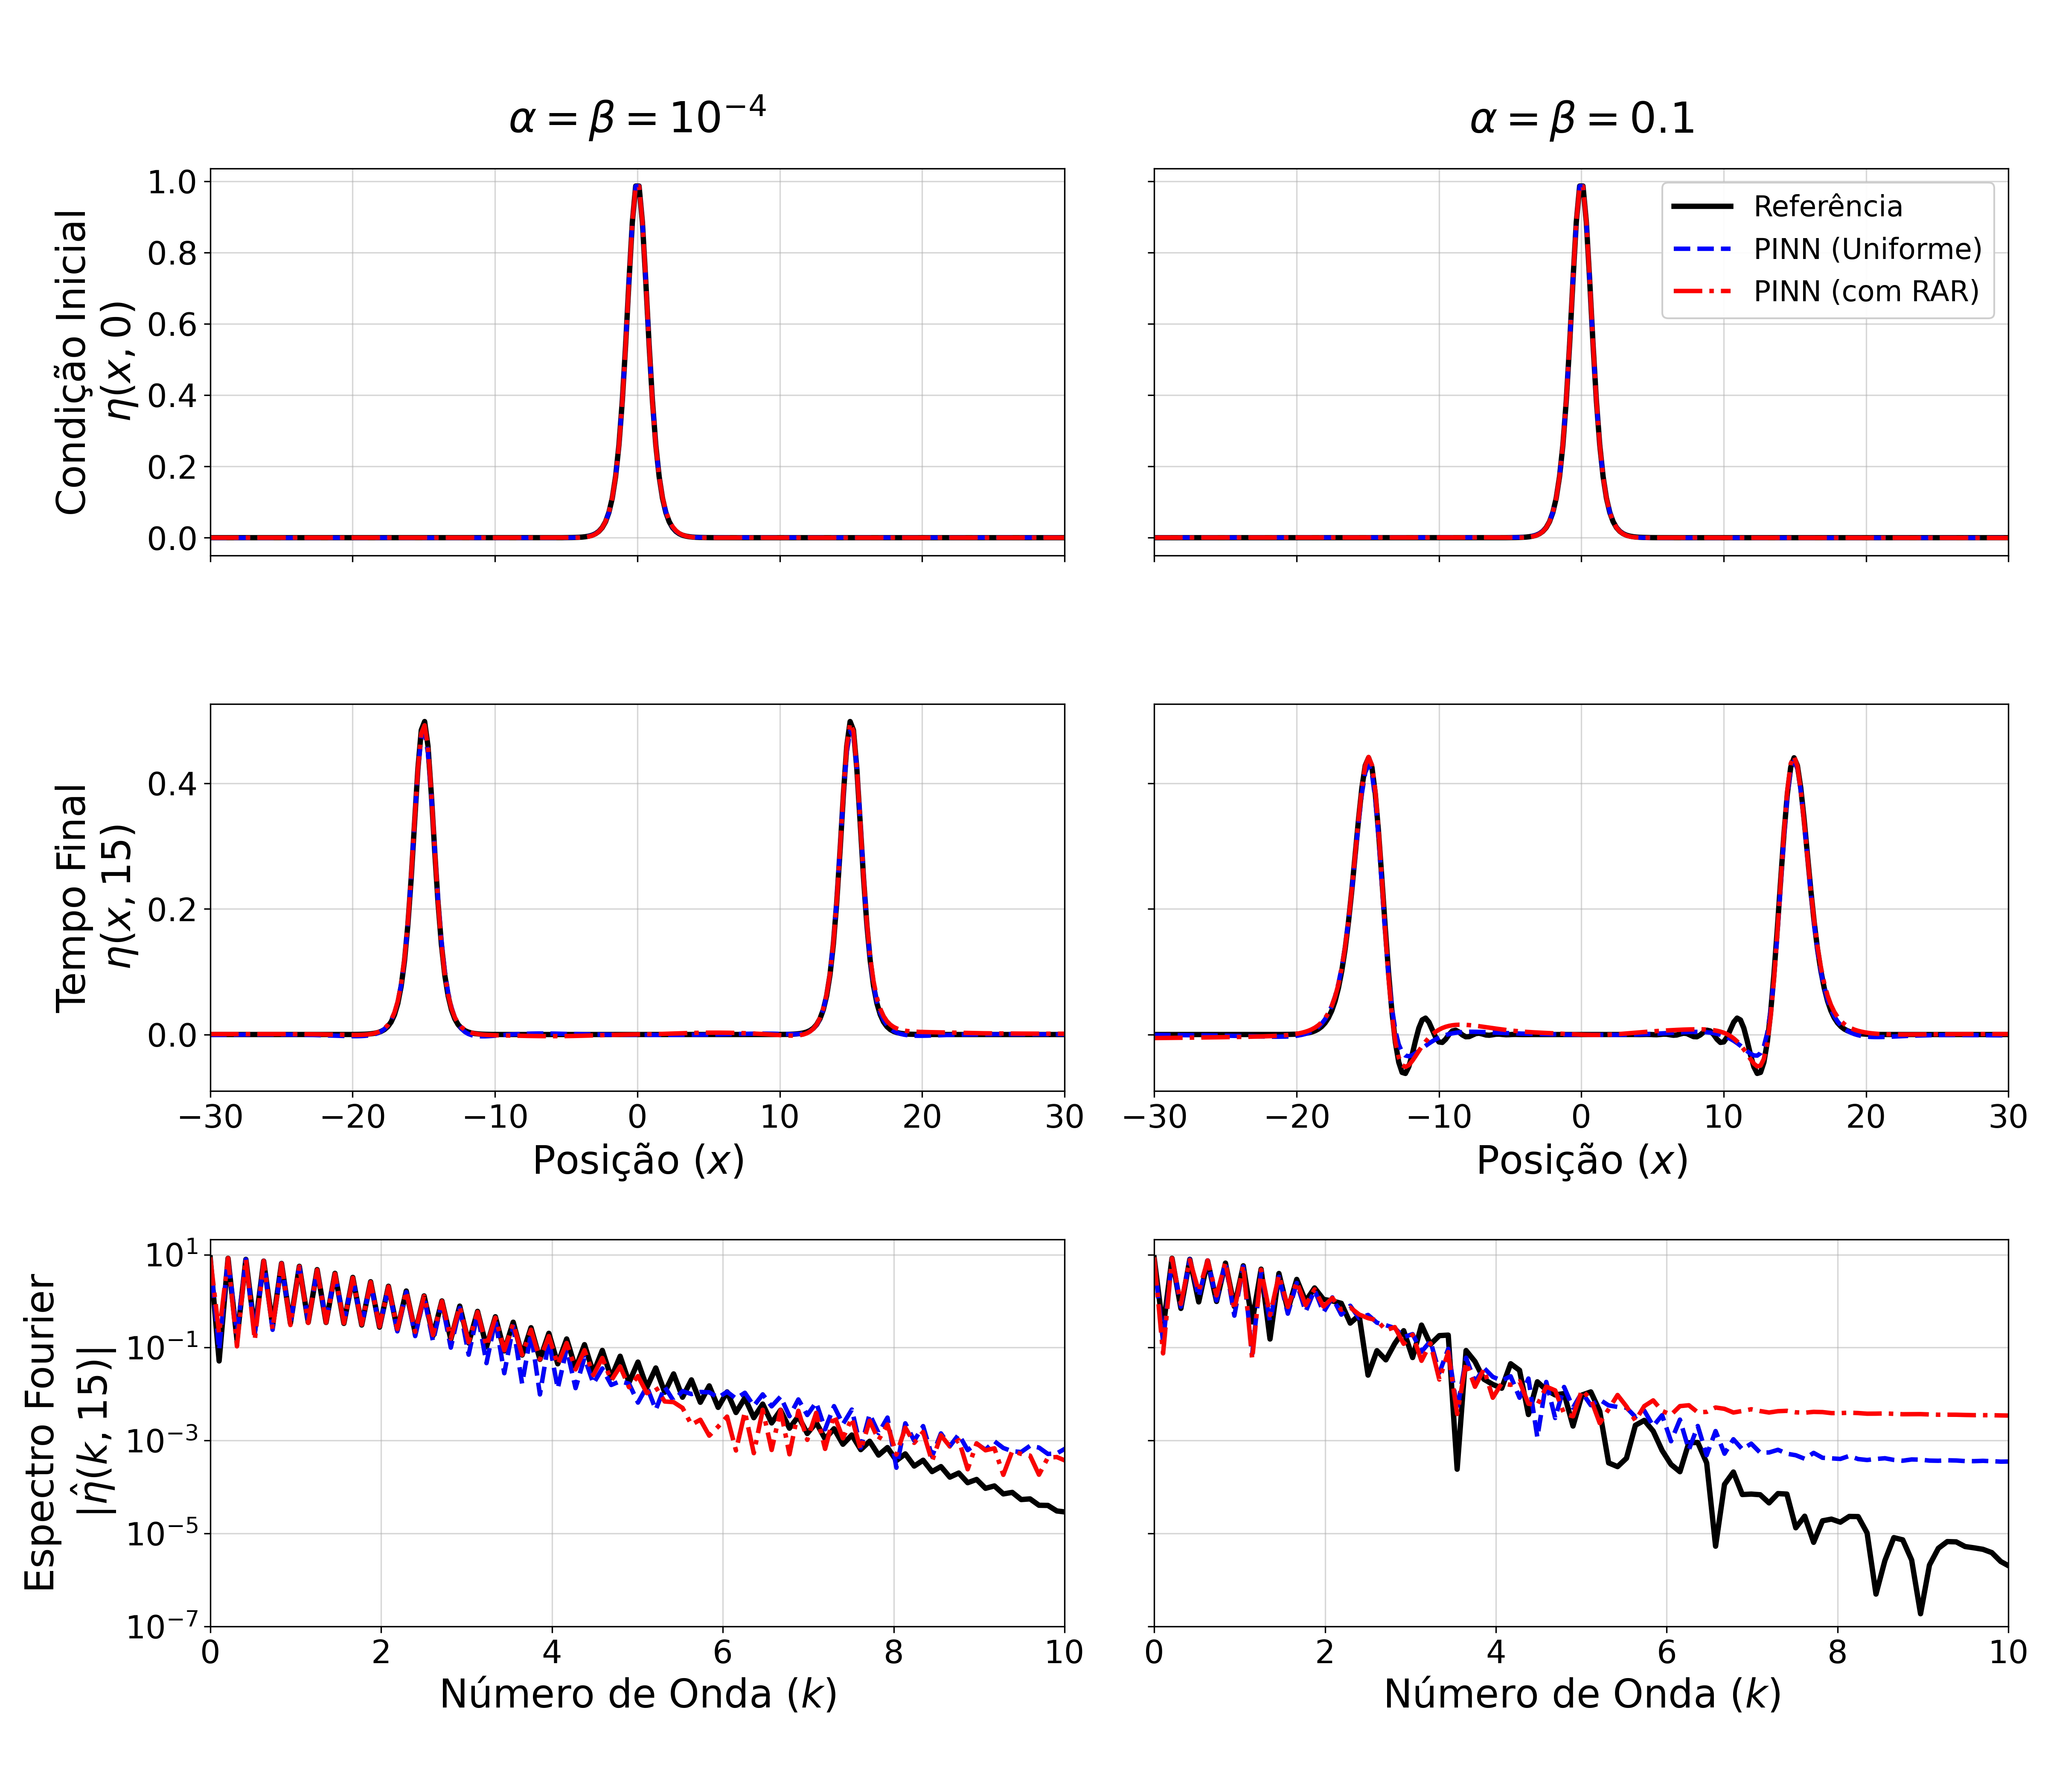
\includegraphics[width=\columnwidth]{imgs/boussinesq_panel_vertical.png}
            \caption{Comparison between PINN solutions (Uniform and with RAR) and the pseudospectral reference for the low ($\alpha=\beta=10^{-4}$, left) and medium-complexity ($\alpha=\beta=10^{-1}$, right) regimes.}
            \label{fig:comparison}
        \end{figure}
        As illustrated in Figure \ref{fig:comparison}, in the regime $\alpha=\beta=0.1$, the approach shows Spectral Bias, indicating that the PINN with uniform sampling (blue) has more difficulty approximating. The PINN with the RAR strategy (red) captures (even if only slightly) the high-frequency components better, getting closer to the reference solution (black), although it does not eliminate the effect completely.
    \end{block}

    \begin{block}{Conclusions}
        This work demonstrated that PINNs have a two-sided performance:
        \begin{itemize}
            \item They are effective in low-complexity regimes, where nonlinear and dispersive effects are mild.
            \item In regimes that are only slightly more complex ($\alpha, \beta$ of significant order), performance is limited by spectral bias and by the difficulty of choosing architectures.
        \end{itemize}
        Adaptive sampling (RAR) proved to be a useful strategy to mitigate this effect, but it does not eliminate it completely. This reinforces that PINNs are an emerging tool, and not a universal substitute for classical methods, requiring further study of their limits.
    \end{block}

    \begin{block}{References}
        \nocite{*}
        \bibliographystyle{plain}
        \bibliography{poster}
    \end{block}

\end{column}
\separatorcolumn
\end{columns}
\end{frame}

\end{document}